
\chapter{Method Of Attack}\label{sec:methodofattack}

After turning on the engine the fan is set to approximately 5000 rpm, which results in a mean velocity of 20.66 m/s in the test section. A LabView program controls the pressure measurements. The actuator moves automatically in radial direction. The distance between two measuring points is 5.5 mm. After measuring the individual pressure of each hole at one circumferential angle $(\Theta)$ (Figure \ref{fig:f4})the probe needs to be moved manually to the next angle where the measurement starts all over again.

\begin{figure}[H]
\centering
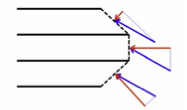
\includegraphics[width=0.3\textwidth]{pics/f4.png}
\caption{Two-dimensional model of the probe tip}
\label{fig:f4}
\end{figure}

 The evaluated range is $22.5\,^{\circ}$ with a step size of approximately $1.125\,^{\circ}$. The data has been saved in a text file and is analyzed in MATLAB. Finally velocity components can be derived from the definition of mach number and geometrical concepts.

